\documentclass[11pt, oneside]{article}   	% use "amsart" instead of "article" for AMSLaTeX format
\usepackage{geometry}                		% See geometry.pdf to learn the layout options. There are lots.
\geometry{a4paper}                   		% ... or a4paper or a5paper or ... 
%\geometry{landscape}                		% Activate for rotated page geometry
%\usepackage[parfill]{parskip}    		% Activate to begin paragraphs with an empty line rather than an indent
\usepackage{graphicx}				% Use pdf, png, jpg, or eps§ with pdflatex; use eps in DVI mode
								% TeX will automatically convert eps --> pdf in pdflatex		
\usepackage{amssymb}
\usepackage{verbatim}
\usepackage{amsmath, mathtools}
\usepackage{amsfonts}
\usepackage{amssymb}
\usepackage{graphicx}
\usepackage{colortbl}
\usepackage{xr}
\usepackage{hyperref}
\usepackage{longtable}
\usepackage{xfrac}
\usepackage{tabularx}
\usepackage{float}
\usepackage{siunitx}
\usepackage{booktabs}
\usepackage{caption}

\hypersetup{
    bookmarks=true,         % show bookmarks bar?
      colorlinks=true,       % false: boxed links; true: colored links
    linkcolor=red,          % color of internal links (change box color with linkbordercolor)
    citecolor=green,        % color of links to bibliography
    filecolor=magenta,      % color of file links
    urlcolor=cyan           % color of external links
}

%% Comments
\newif\ifcomments\commentsfalse

\ifcomments
\newcommand{\authornote}[3]{\textcolor{#1}{[#3 ---#2]}}
\newcommand{\todo}[1]{\textcolor{red}{[TODO: #1]}}
\else
\newcommand{\authornote}[3]{}
\newcommand{\todo}[1]{}
\fi

\newcommand{\wss}[1]{\authornote{blue}{SS}{#1}}
\newcommand{\ms}[1]{\authornote{red}{Malavika}{#1}}

\newcounter{funcnum} %Functionality of Issue Tracking System
\newcommand{\athefuncnum}{P\thefuncnum}
\newcommand{\fref}[1]{F\ref{#1}}

\newcounter{insnum} %Instructions of  Issue Tracking System
\newcommand{\atheinsnum}{P\theinsnum}
\newcommand{\iref}[1]{I\ref{#1}}

\begin{document}

\title{Instruction Manual for Issue Tracking} 
\author{Malavika Srinivasan, Spencer Smith, and Dan Szymczak}

\date{\today}

\maketitle

\wss{In the title, please use capital letters to start the important words
  (Instruction Manual for Issue Tracking).}
  \ms{Changed title.}

\tableofcontents
\newpage

\section{Introduction to GitLab} \label{Introduction}

The primary goal of this document is to provide a set of instructions to use the
issue tracking system in Gitlab.  GitLab is a software or a free repository
manager with an open source license. GitLab comes with many features like -
repository management, code reviews, issue tracking, activity feeds and
wikis. GitLab is often used for continuous integration and delivery. In this
manual, we will deal with `issue tracking', which is the set of activities
associated with scheduling and reviewing a task. It is described in detail in
the Section~\ref{Issue_Tracking}.

\wss{Use a capital letter for Section, just like you do for Figure.}
\ms{Changed "section" to "Section"}

\subsection{Issue Tracking}\label{Issue_Tracking}

An Issue Tracking System (ITS) is a computer software package that manages and
maintains lists of issues. The ITS provides the necessary infrastructure to
create, update, and resolve (close) issues.

\subsubsection{Issues}

Issues are set of tasks assigned to be completed. Each issue in the system may
have an urgency value assigned to it, based on the overall importance of that
issue. Low or zero urgency issues are minor and should be resolved as time
permits. Besides this for each issue, the date of submission, detailed
descriptions of the issue, attempted solutions or work-arounds, and other
relevant information are also recorded by the ITS.

\subsubsection{Functionality of ITS}

Issue Tracking System has its own set of functionality:

\begin{itemize}

\item[F\refstepcounter{funcnum}\thefuncnum \label{f_one}:] Creation and
  allocation of tasks easily.
\item[F\refstepcounter{funcnum}\thefuncnum \label{f_two}:] Monitoring of
  handling, time spent and quality of work.
\item[F\refstepcounter{funcnum}\thefuncnum \label{f_three}:]Assignment of a
  priority to each issue based on the overall importance of that issue.
\item[F\refstepcounter{funcnum}\thefuncnum \label{f_four}:]Containing a detailed
  descriptions of the problem being experienced, attempted solutions or
  workarounds, and other relevant information.
\item[F\refstepcounter{funcnum}\thefuncnum \label{f_five}:]Maintaining of a
  history of each change.

 \end{itemize}

\clearpage

\subsubsection{Instructions for Issue Tracking System}

\begin{itemize}

\item[I\refstepcounter{insnum}\theinsnum \label{i_one}:] Go to the url -
  \url{https://gitlab.cas.mcmaster.ca} and enter your login and password as
  shown in the Figure \ref{Fig_img1} .

  ~\newline
\begin{figure}[ht]
\begin{center}
\caption{\label{Fig_img1} Steps in Issue Tracking}
 % rotatebox{-90}
{
 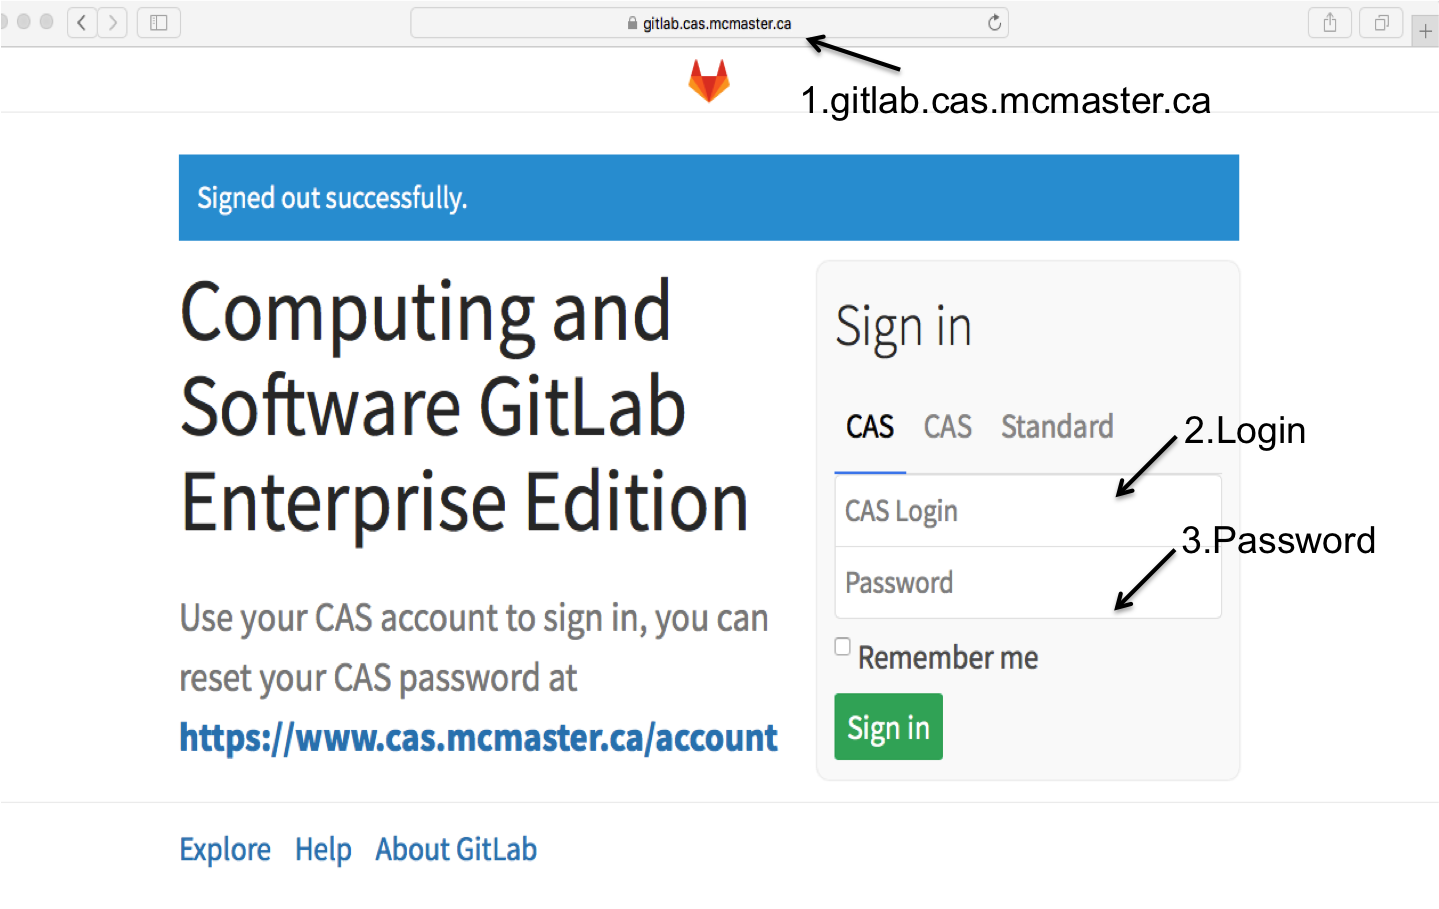
\includegraphics[width=1.00\textwidth]{img1.png}
}
\end{center}
\end{figure}
\clearpage

\item[I\refstepcounter{insnum}\theinsnum \label{i_two}:] Choose
your group's repository.

\item[I\refstepcounter{insnum}\theinsnum \label{i_three}:] Choose the option
\textbf{Issues}.

%\item[I\refstepcounter{insnum}\theinsnum \label{i_four}:] Click
%\textbf{Label} and choose a label to display only issues with that label.


\item[I\refstepcounter{insnum}\theinsnum \label{i_five}:]To create a
              new issue, choose \textbf{New Issue} as shown in Figure
              \ref{Fig_img5}.

\begin{figure}[ht]
\begin{center}
\caption{\label{Fig_img5} Steps in Issue
  Tracking}
%rotatebox{-90}
{
 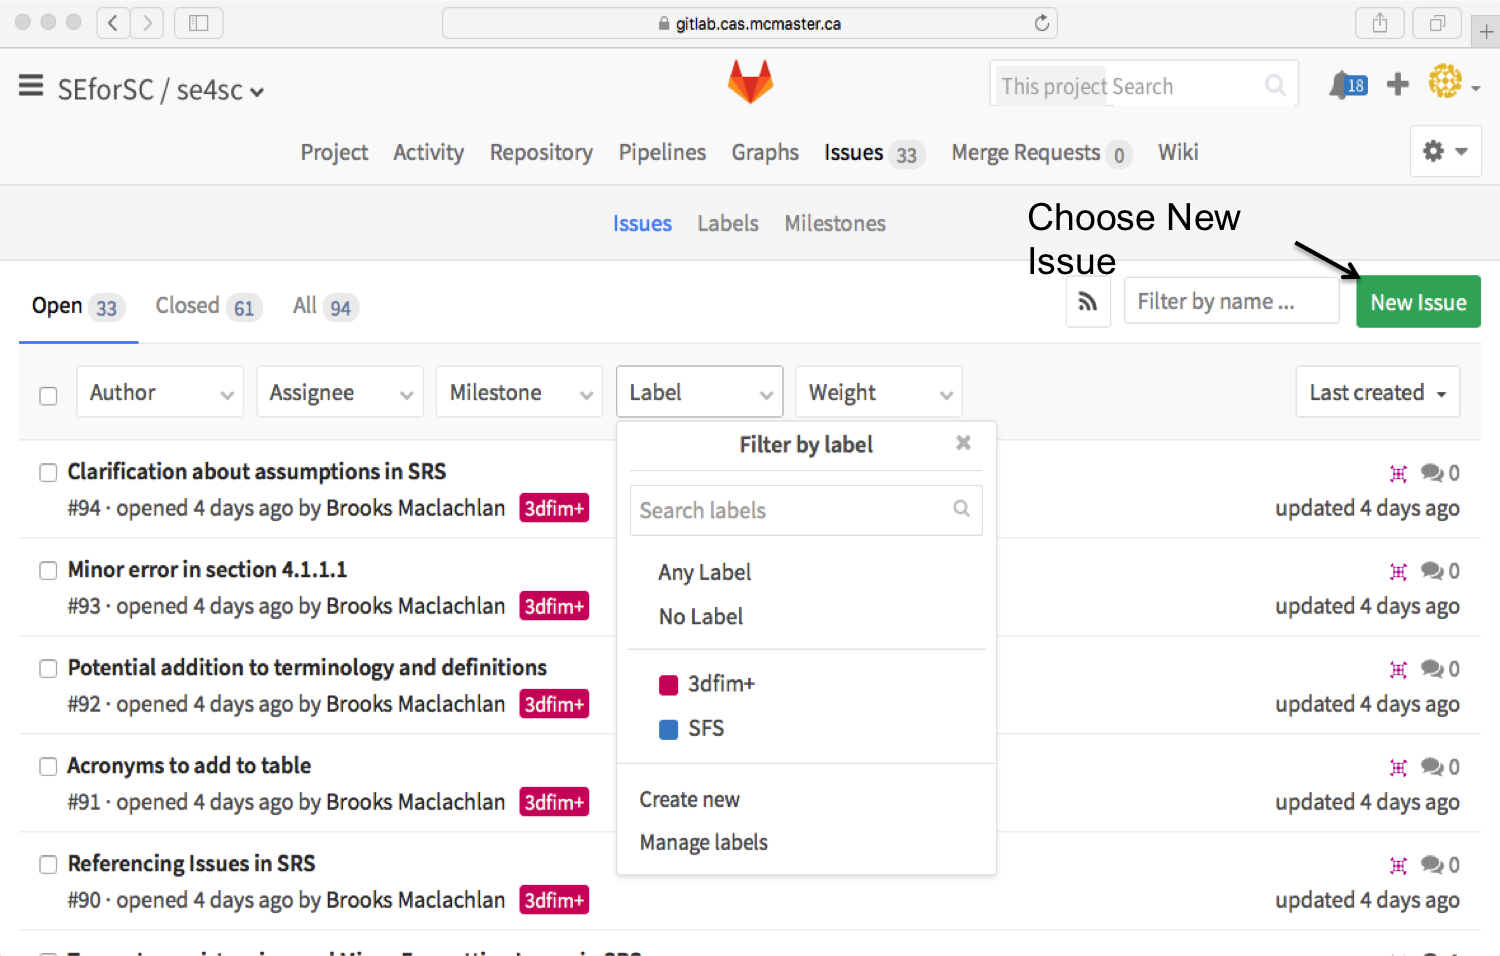
\includegraphics[width=1.00\textwidth]{img5.png}
}

\end{center}
\end{figure}


\item[I\refstepcounter{insnum}\theinsnum \label{i_six}:] Fill in
                  the necessary fields like Title, Description, Assignee, Labels
                  etc.\ and click \textbf{Submit issue}.

                  Note: \# symbol can be used to reference other issues and @
                  symbol can be used to reference other users. Also, you can
                  reference specific commits by using their SHA-hash.


\item[I\refstepcounter{insnum}\theinsnum \label{i_seven}:] To
                  comment on an issue, write a brief description of your comments, then click ``Comment''.

\item[I\refstepcounter{insnum}\theinsnum \label{i_eight}:] To
                  close an issue, go to the issue's page and write a brief
                  description of what you did to close the issue, then click
                  ``Comment \& close issue''.

\end{itemize}

\subsubsection{Markdown}

From \href{https://guides.github.com/pdfs/markdown-cheatsheet-online.pdf}{https://guides.github.com/pdfs/markdown-cheatsheet-online.pdf}:
``Markdown is a way to style text on the web. You control the display of the
document; formatting words as bold or italic, adding images, and creating lists
are just a few of the things we can do with Markdown. Mostly, Markdown is just
regular text with a few non-alphabetic characters thrown in, like \# or *.''

You can use Markdown syntax to add headers, lists, emphasis, emojis etc.  When
you get started Markdown is optional, but as you gain experience, you will
likely find that you are using it to improve the expressiveness of your text.

\subsubsection{Milestone}

GitLab and GitHub also support entering dates for milestones.  You might want to
add your course deliverables as milestones.

\end{document} 